%% Please put your respective section title as input as the first comment 

%% Step 1: make a folder of your name under sections folder 
%% Step2 : make a .tex file of each section and include in this current file as shown bellow:
%\input{sections/<you_name>/<section_title>}
%% Step 3: In case of adding images make a directory under your name in images folder and put all the images in your directory. Then add the figure in your section according to image path.
%% sample figure syntax::
% \begin{figure}[h]
% \includegraphics[scale=0.7]{images/<your_name>/<image_name>.jpg}
% \centering
% \label{fig:<figure_name>}
%\end{figure}
% for adding bibliography please add references on a .bib under your name in bibliography folder
\subsection{Definition [Md Anisul Haque]}
%
CI/CD comes forward to automate software production via continuous integration and continuous delivery more frequently and efficiently.

Continuous integration (CI) and continuous delivery (CD) are the base concepts that are allowed to cope up with any changes, like code change, configurations, data, environments etc, for the entire production road\cite{CD}.

Nowadays, software industries are paying the highest intention to automation developments. In a competitive market, whoever delivers a product on the fly is ahead of those who lag in productions. CI/CD is faster than releasing big batches of updates and patches all at once as any part is not bound on other's work. It also ensures that products are published faster, are more up-to-date, and have improved security and scale, all of which are essential aspects of agile networking.

CI is the process where the source is being developed and tested simultaneously in a continuous manner, whereas CD provides the mechanism that makes a usable version for end users\cite{CDHandsOn}.

"Continuous integration is a coding philosophy and set of practices that drive development teams to implement small changes and check-in code to version control repositories frequently. Because most modern applications require developing code in different platforms and tools, the team needs a mechanism to integrate and validate its changes." \footnote{https://www.infoworld.com/article/3271126/what-is-cicd-continuous-integration-and-continuous-delivery-explained.html}

%
\subsection{Components [Md Anisul Haque]}
%
A CI/CD pipeline is made up of distinct subsets of tasks that are known as pipeline components. The following are the most common pipeline components:

\subsubsection{Development}

Basically, it is the start point of the pipeline; whenever any changes are pushed its automatically got triggered. The development phase is dependent on language and technologies, which is a prerequisite for decision-making before starting deployable units. For example, in JAVA, tools like Maven or Gradle are necessary to build a JAVA distribution. A packaging phase may include the automated build elements. Taking the JAVA example a step further, if a Docker Image of the JAVA app is needed, the required Docker Compose steps must be called. Build-centric tests, such as unit tests and dependency scanning, can be performed in the build components.\footnote{https://harness.io/blog/continuous-delivery/ci-cd-pipeline/}


The compilation is required for programs written in languages like Java, C/C++, C\# or Go, while Ruby, Python, and JavaScript do not. Cloud-native software is usually deployed with Docker, so this stage of the CI/CD pipeline creates Docker containers, regardless of the language. Failure to pass the construct stage indicates a fundamental problem. And for a successful release, a successful development phase is must.\footnote{https://semaphoreci.com/blog/cicd-pipeline}


\subsubsection{Testing}
Testing as name referred, here build product undergoes testing. Testing can be done partly or as a whole. However, the best practice is to test partly because failing on part or unit test demolishes the need for a total integration test, which saves both time and effort. The test can be like integration tests, soak tests, load tests, and regression tests, all of them has their own significance.\footnote{https://harness.io/blog/continuous-delivery/ci-cd-pipeline/} Integration test is the test where all modules are connected and tested as a whole group. Soak tests are more likely to test on a particular load over some specific period to determine an approximation of real-time use. Load test is checking response under some specific pressure. Regression tests are used to determine whether it's working or not with the new release. There are some more tests like functional tests, unit tests, and performance tests etc. All of them ensure the quality of the solutions. Here the main advantage is the early error detection instead of waiting for a complete production release. The QA team identifies problems than reported the concerns with feedback. Based on the priority, respective teams make feasible solutions. Again, these go for testing chain upon successful build.


\subsubsection{Release}

The successful release is the prerequisite for successful deployment. The continuous release makes it grow more confident in deployment. It is the point where any new or changed features are ready to deliver to the repository. Release components are the individual implementations that help achieve Continuous Implementation. The most common release techniques are Rolling, blue/green and canary deployments.\footnote{https://harness.io/blog/continuous-delivery/ci-cd-pipeline/}

  
\begin{itemize}
    
\item \textbf{Rolling Deployment}: Rolling deployment works on a distributed system, contains multiple server or clouds instance. All of them carry the application simultaneously. But here, the update took place sequentially, so some may get the update earlier than others. Meanwhile, some users may experience the new version and end of the circle; everyone will get the same version. Here rollback is more accessible, but testing needs a longer time as it works like one by one release.
    
    
\item \textbf{Blue-Green Deployment}: Blue-Green deployment consists of two deployment units, blue is for staging and green for production. New releases are being deployed in blue units, and after testing or finalizing, the green one is pointed, and blue goes to the public. Here also rollback is easy but costing is higher as both the unit have the same environment.
     
    
\item \textbf{Canary Deployment} : Canary deployment divides distribution in some sets. New releases are first deployed on a set of servers. Furthermore, upon their successful feedback, this release was then deployed on the next set, eventually on every set. For example, the first phase would swap 25\% of the nodes, and if successful, the second phase would swap 50\% of the nodes, and the third phase would swap 100\% of the nodes. The stability they offer during a release and the fact that they use fewer resources than a blue-green deployment are the reasons for implementing canary deployments. Here the main advantage is the early feedback from the user or tester, which makes the application more efficient \cite{inproceedingsMunch}.
  
\end{itemize}


\subsubsection{Deployment}

Deployment is the final step of CI/CD pipeline. As soon as the testing phase validates, it should go for deployment. In CI/CD deployments are small updates are delivered continuously. This process is automated. It removes so many manual efforts. Here version is maintained and added to the solution and further feedback is gathered in correspondence to these versions. Most of the works have already been done by previous steps and in deployment, it is more likely one time job to configure in a suitable way that will follow upcoming deployments.\footnote{https://cinglevue.com/how-to-build-an-efficient-ci-cd-pipeline/}


%
\subsection{CI-CD on Cloud [Md Anisul Haque]}
%
Here CI/CD on cloud refers, the complete mechanism of the CI/CD is maintained and hosed via cloud service. Although cloud computing has multiple meanings, the most basic definition is a framework that allows and facilitates the provisioning of resources. It can be private or public. There are various cloud CI/CD providers like Azure, AWS, Google cloud etc., all of them have their own services\cite{inproceedings}. The efficient structure of cloud computing is one of the most significant advantages of the cloud for CI/CD. This is ideal for CI/CD workloads, which are ephemeral and burst. Cloud services can scale up and down dynamically in response to CI/CD workloads. For enterprises, this provides significant management and cost savings. Enterprise firms do not need to run their own servers, but they do need to scale up as CI/CD workloads grow, and they don't want to spend server resources when they're not in use. Cloud can be private in a scene that if the company has own data center and all other resources to accomplish the entire pipeline task. Here, it might not be possible to facilitate every need, like the product might need sudden high distribution for the load or limitations of storage power or even speeds for geographic diversity. The private cloud is mainly used for high security and high sensitive data issue. However public cloud host all the solutions, providing high security and scaling facility like load balancing , storage on demand, geographical location based distribution and so on. The hybrid cloud is a more modern approach that combines private and public cloud services. Depending on needs, the system can go for the private or public one. The best thing is that the cloud provides so many benefits like low costing for the architecture, certified security system, easy data management, high flexibility, low configuration, reliable service, supports from global developers, etc. 
\footnote{https://devops.com/cloud-and-devops-ci-cd-and-market-analysis/}
%
\subsection{Different Tools for CI-CD on Cloud [Md Anisul Haque]}
%
There are so many tools available for CI/CD on the cloud. Namely Azure DevOps, AWS, Google Cloud and so on. All of them have their own significance. 
%
\subsubsection{Azure DevOps}
%

Azure DevOps is the most popular Software as a Service (SaaS) platform from Microsoft provider. It is flexible as here services can be taken on the basis of need. It is platform-independent and compatible with any language. There are various services in Azure such as Azure Repos, Azure Pipelines, Azure Boards, Azure Test Plans, Azure Artifacts etc. It also has an instance of git named Azure git for version control. Azure repo is just taken care of it. Azure boards follow the agile methodology and are able to prepare reports on bugs or other issues. It is also compatible with AWS and Google Cloud. The whole process is as simple as, first we make an organization, then create a new project. After that, create the pipeline with the YML file. The next step is authorization and finally, approve and run the pipeline. These are the basic steps to configure the Azure pipeline.

%
\subsubsection{AWS}
%

AWS CodePipeline is a professional automated continuous distribution service that facilitates automating the release pipelines for fast and stable device and infrastructure updates. CodePipeline automates the develop, test, and deploy phases of the release process based on the defined release model whenever there is a code update. This makes it possible to offer features and upgrades quickly and consistently. AWS CodePipeline can be seamlessly integrated with third-party platforms like GitHub and many custom plugins. Users have to pay for what they use with AWS CodePipeline. There are no hidden costs or long-term obligations. There are many advantages in AWS such as rapid delivery, configurable workflow, get started fast, easy integration etc.\footnote{https://aws.amazon.com/codepipeline/}


%

\subsubsection{Google Cloud}
%
In the public cloud industry, Google Cloud Platform is one of the most common cloud providers. It offers various managed services, and it makes sense to use Google Cloud's managed CI/CD software if you are solely using Google Cloud.\footnote{https://medium.com/swlh/how-to-ci-cd-on-google-cloud-platform-1e631cded335} One of the core principles of the google cloud platform is its commitment to open-source development support. Many of the features of GCP are developed by the community and are easy to integrate into the GCP Platform, which makes it easier to get support for an application. Even though Google got into the cloud market later than its counterparts, its commitment to open-source development is helping them grow their offered features exponentially.  
%


%
\subsection{Technical Overview of AWS [Md Saiful Ambia Chowdhury]}
%
There are numerous products and services are offered by AWS to facilitate the development, production, and maintenance of a software system. These include computing, storage, database, networking, application services, deployment, management, analytics, machine learning, developer tools, IoT tools, and so on. Among these, the most popular are Amazon ElasticCompute Cloud \textbf{(EC2)}, Amazon Simple Storage Service \textbf{(Amazon S3)}, Amazon ElasticBlock Store \textbf{(EBS)}, Amazon Connect, and AWS Lambda. Down below, a brief description of the AWS services related to CI/CD is given.\footnote{https://aws.amazon.com/products/developer-tools/?nc2=h\textunderscore ql\textunderscore prod\textunderscore dt}.

\subsubsection{Amazon Elastic Computing Cloud (EC2)}
%
EC2 is one of the most reliable IaaS available nowadays, provided by AWS. It allows users to create and access a virtual cluster of computers according to their need for CPU power, amount of memory, storage, OS, and other resources. Users can boot an Amazon Machine Image (AMI) along with their preferred software. Amazon refers to the AMI as 'Instance.' Amazon EC2 supports Linux, Windows Server 2012, CentOS 6.5, and Debian 7.4.
%

\subsubsection{AWS CodeCommit}
%
AWS provides a fully-managed source control service named AWS CodeCommit. It can be used as our own private Git repositories in a secured environment that is managed by AWS. The AWS CodeCommint supports all the features of a git-based source control system and can be managed by all the existing Git client tools. It is the first step to build a CI/CD pipeline with AWS.  
%

\subsubsection{Amazon S3}
%
Amazon S3 s for Amazon Simple Storage Service, and its sole purpose is for object storage. It supports the typical folder structures and all the common file types. Amazon S3 has a built-in redundancy that copies our object across three availability zones.
%

\subsubsection{AWS CodeBuild}
%
Amazon provides the continuous integration service through the service called AWS CodeBuild. With CodeBuild, we can compile our source code, run tests, and build deployable artifacts. Users can build their application with all the popular programming languages and build tools such as Apache Maven, Ant, Gradle, etc. It also supports multiple builds parallelly and automatic scaling of the server.   
%

\subsubsection{AWS CodeDeploy}
%
To automate the application deployment process into Amazon EC2 as well as on-premises servers, Amazon provides the AWS CodeDeploy service. Using CodeDeploy, one can eliminate the need for tedious and error-prone manual deployment operations. Thus it became possible to reduce the downtime during the deployment process and provide quick release. Other advantages of using CodeDeploy include centralized monitoring and controlling with AWS CLI, SDKs, or APIs, tracking deployment histories, and maintaining multiple deployment groups.  
%

\subsubsection{AWS CodePipeline}
%
In order to automate our code release process from local development to production, Amazon offers AWS CodePipeline. This CodePipeline allows us to design, visualize and run the required steps for deployment automatically for our software release. A pipeline can be started manually, also can be triggered with a change in the source code. Using the Amazon CloudWatch Events, we can trigger the execution of a pipeline upon any push into the repository. \footnote{https://docs.aws.amazon.com/codepipeline/latest/userguide/concepts-continuous-delivery-integration.html}
%

\subsubsection{AWS CloudFormation}
%
AWS CloudFormation is an IaaC service provided by Amazon. With AWS CloudFormation, Amazon helps its customers to spend little time managing and provisioning other AWS resources such as EC2, AWS S3, etc. To use this service, the user can describe the resources along with the attributes in a template file, from which AWS CloudFormation manages the infrastructure and detects changes. 
%

%
\subsubsection{CI-CD Process using AWS}
%
In this section, we will explore a simple implementation of CI-CD using AWS services. To demonstrate this example, we need two separate AWS accounts- one for development and one for production. At first, we will set up the AWS CodeCommit repository with our source code. It is also required to schedule a CloudWatch event with CodePipeline so that any changes in the source code will trigger the Pipeline. Then the Pipeline will fetch the changes from the repository and try to build the application with AWS CodeBuild. After a successful build, CodeBuild will run the provided unit tests and stores the artifacts into the Amazon S3. If everything is a success, the Pipeline will deploy the application in the development account. Upon a successful deployment on the development account, the Pipeline triggers the deployment in the production account. We can also configure this deployment to be activated manually for authorization and security. \footnote{https://aws.amazon.com/blogs/devops/complete-ci-cd-with-aws-codecommit-aws-codebuild-aws-codedeploy-and-aws-codepipeline/}:

The following diagram illustrates the workflow:

\begin{figure}[h]
    \centering
    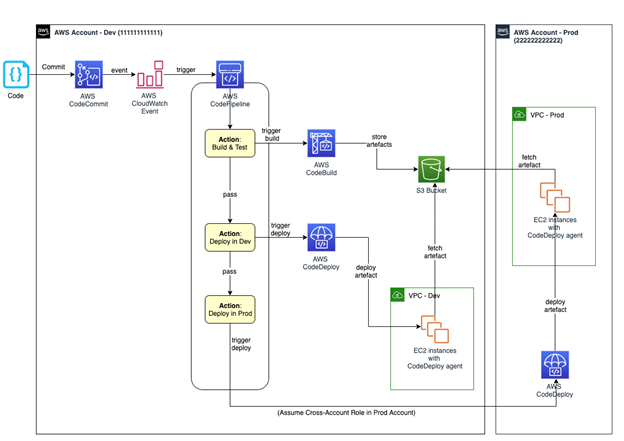
\includegraphics[width=\textwidth]{images/saiful/aws_cicd.png}
    \caption{Workflow of CI/CD pipeline in AWS.}
    \label{fig:aws_cicd}
\end{figure}

%

\subsubsection{Estimated Cost}
%
Amazon follows a 'pay as you go model to charge its clients. A user only needs to pay when he uses any of the resources or services. Additionally, many of the services offer some basic free trials, which are very useful for testing simple applications. Though, we can say the pricing structure can be a bit complicated for complex applications using various AWS services.\cite{AWS_Cost} The cost can be calculated based on the usage and configuration of the CI/CD pipeline and other resources using the AWS Pricing Calculator (https://calculator.aws/). With the basic configuration of the resources and services mentioned in the previous section, an estimated \$15 per month bill can be expected.\footnote{https://aws.amazon.com/getting-started/projects/set-up-ci-cd-pipeline/services-costs/}
%

\subsubsection{Advantages}
%
AWS is a fast-growing cloud provider for its several advantages. Both individuals and organizations are moving into AWS services for its simplicity, flexible pricing plans, and other facilities. AWS provides a user-friendly UI, which makes it very simple to use for new users. It also provides state-of-the-art security and reliability for all of its resources. The Auto Scaling service automatically adjusts the capacity of the resources. The scalability and elasticity include both downscaling and upsizing. With the pay-as-you-go pricing structure, the users have to pay less and only for the duration of usage. With the rapidly growing network of AWS over the world, the scope of operation is also expanding with more availability. AWS is offering more and more services targeting the needs of the users.



%


\subsubsection{Disadvantages}
As everything has its limitations, Amazon Web Services comes with a few disadvantages. Some may find it difficult to calculate the overall cost for a large company using numerous AWS services. An essential fact for keeping the cost minimum is to utilize the resources efficiently. Additional charges may be applied for technical supports, which differs for different consumer types. There are also some differences between the default limits on the same resources in different regions. AWS offers several similar services that make the users overwhelmed while choosing the right services for their needs.






%

%
%
\subsection{Technical Overview of GCP [Shoaib Bin Anwar]}
%
Google Cloud Platform is one of the most used public cloud platforms and is still continuing to grow. It offers a cloud services that run on same infrastructure that Google hosts their product such as Google search, Gmail and Youtube. After Launching of Google App Engine, we have seen other services introduced and the list is continuing to rise.
%
% \subsection{CI-CD Process}
%
% How to setup CI-CD on the tool?


\subsubsection{Setting up a CI/CD pipeline for data-processing workflow}
%
Setting up a continuous integration/continuous deployment is done by implementing CI/CD methods with manage products on Google cloud. The methods are version control (git), build, test and deploy of application, and isolate production environment from  development and staging environment.
%
\subsubsection{Deployment Architecture}
%
\begin{itemize}
    \item  \textbf{Cloud Build} is a service to create CI/CD pipelines for building, deploying, and testing.  It is a series of steps and each step is run in Docker Container. 
    \item \textbf{Cloud Composer} is used for users to manage entire Google Cloud Platform (GCP) pipeline which includes create, schedule, monitor, and manage complex workflows.
    \item \textbf{Dataflow} is the server-less execution service from GCP for data-processing pipelines written using Apache Beam. Apache Beam is an open-source, unified model for defining both batch and streaming data-parallel processing pipelines.
\end{itemize}

\subsubsection{The CI/CD pipeline of GCP}
%
 Cloud Build packages the sample application into a JAR file using the Maven Builder or Gradle Builder. Both are container with Maven or Gradle  installed in it. They run the task when a build step is configured. Cloud Build uploads the JAR file to cloud storage, runs unit tests on data-processing workflow code and deploys the workflow code to the Cloud Composer. Then Cloud Composer picks up the JAR file and runs the data-processing job on Data-flow. 


% 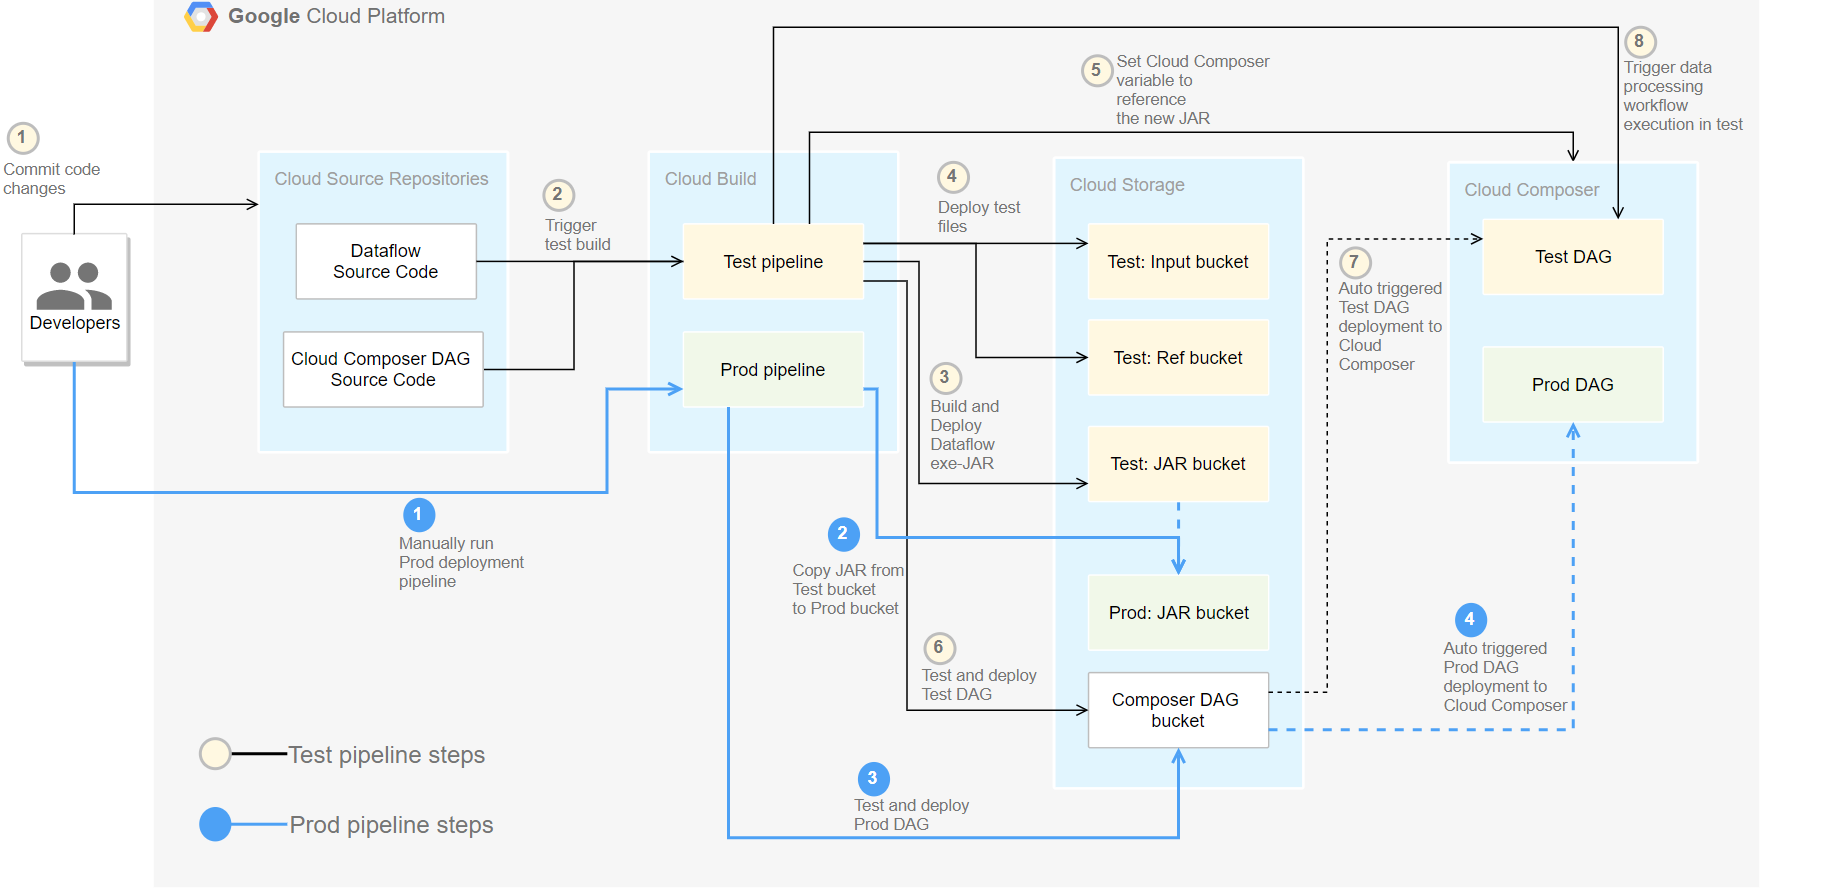
\includegraphics[scale=0.55]{images/shoaib/cicd-pipeline-for-data-processing-1-diagram-pipeline.png}

\begin{figure}[h]
    \centering
    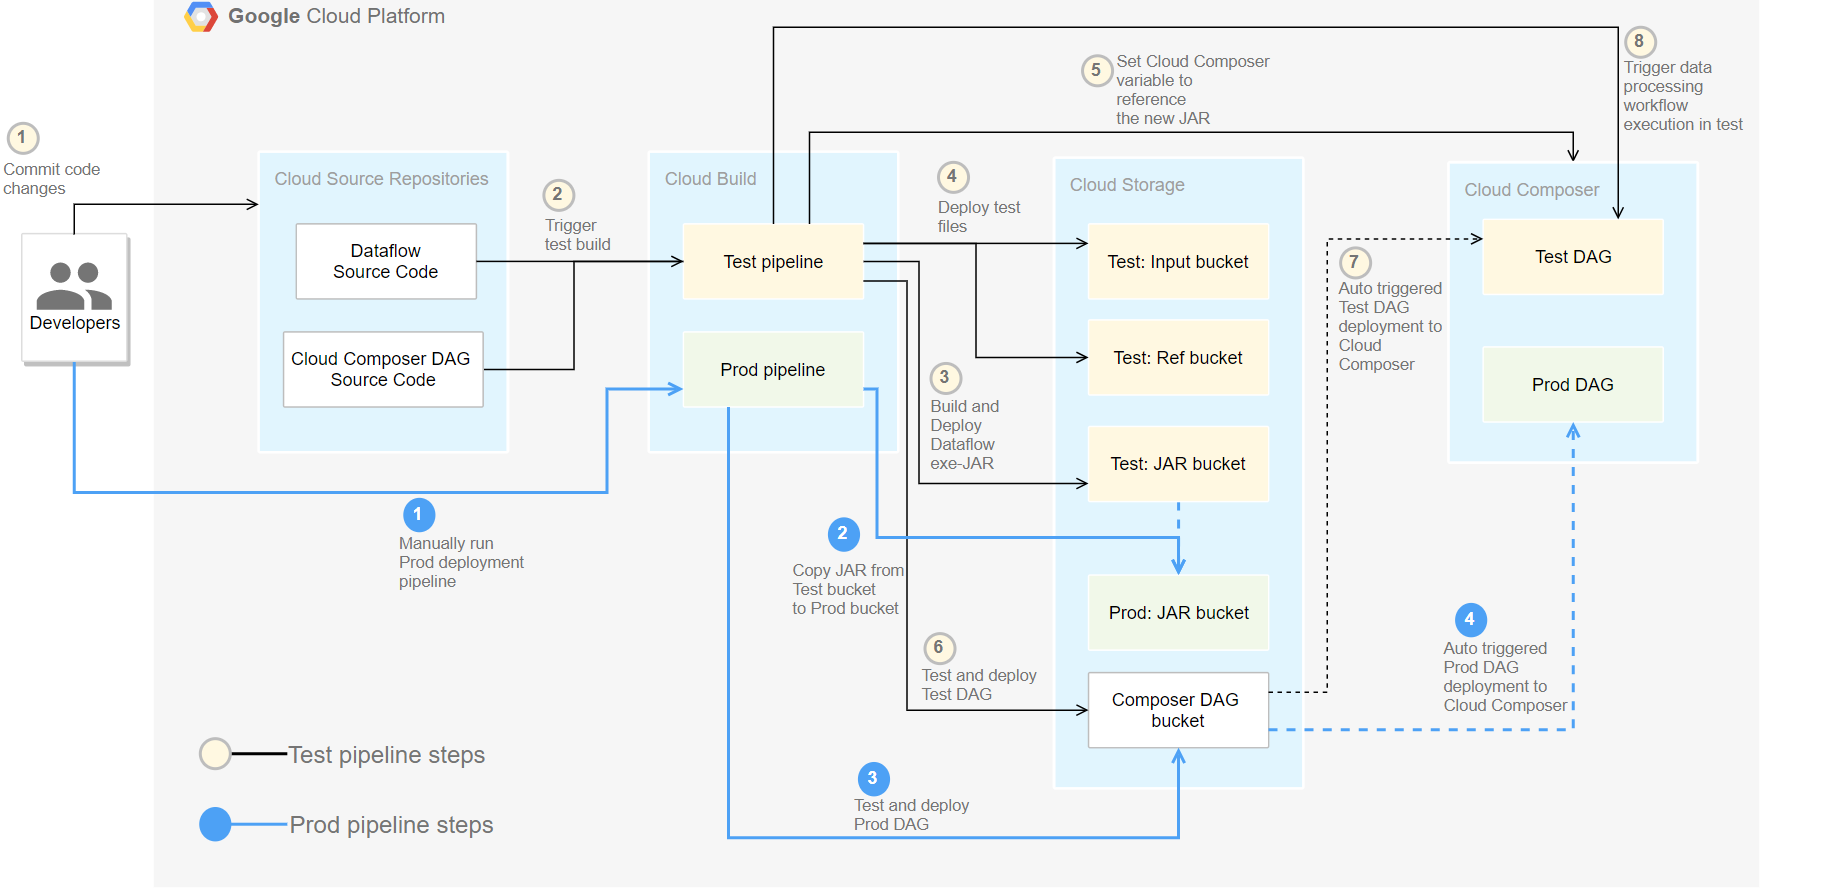
\includegraphics[scale=0.53]{images/shoaib/cicd-pipeline-for-data-processing-1-diagram-pipeline.png}
    \caption{Workflow of CI/CD pipeline in GCP.} 
    \label{fig:gcp_cicd}
\end{figure}
%
We can see in the figure~\ref{fig:gcp_cicd},  the deployments to the test and production environments are separated into two different cloud Build pipelines- a test and a production pipeline.\footnote{https://cloud.google.com/architecture/cicd-pipeline-for-data-processing\#the\_cicd\_pipeline} 
\newline In test pipeline, from the figure we can see that if developer commits something in the code repository, it triggers a test build in Cloud Build. Then Cloud Build builds JAR file and deploys it to the test JAR bucket on Cloud Storage. At the same time, Cloud Build deploys the test files to the test-input bucket and test reference bucket on cloud storage. Cloud Build also sets the variable to reference new JAR file. It also tests DAG and deploys it to the Composer DAG bucket and then DAG file is deployed to Cloud Composer Test DAG. Finally, Cloud Build triggers data processing workflow execution in test. 

On the other hand, in the production pipeline, developers run production deployment pipeline manually. Cloud Build copies the JAR from Test bucket to Production bucket and tests the DAG and deploy the DAG to the Composer DAG bucket. Then, the DAG file is deployed to Cloud Composer. 


%
%
\subsubsection{Pricing}
%
Google Cloud Platform has no up-front costs, pay-as-you-go services, and no fees for termination. In addition, GCP stands out for for its discounts. 
%
\subsubsection{Advantages}
%
GCP probably benefits from the simple fact that Google owns it. Apart from that, there are some benefits of using GCP. Google Cloud Platform(GCP) is designed for cloud-native businesses and is committed to open source and portability. The other significant advantage is price advantages over the other cloud providers, along with frequent discount offers. 


%
\subsubsection{Disadvantages}
%
GCP has disadvantages like other cloud platform. One of the disadvantages is that GCP is still growing. It has fewer features if we compare it with AWS and Azure. Another disadvantage is about the documentation of GCP as it lacks visual description along with textual descriptions\cite{inproceedingss}. We know that visual description like diagram helps the developer to understand the flow of work. So, it is very difficult for the readers to understand the documentation without enough graphs and diagrams.
%

%
\subsection{Technical Overview of Microsoft Azure}
%
Microsoft leveraged its constantly-growing worldwide network of data centers to create Azure, a cloud platform that facilitates building, deploying, and managing services and applications anywhere. At its core, Azure is a public cloud computing platform—with solutions including Infrastructure as a Service (IaaS), Platform as a Service (PaaS), and Software as a Service (SaaS) and we can use these for services such as analytics, virtual computing, storage, networking, and much more. These services are used to supplement an on-premise server or replace it.

A CI-CD architecture is implemented in Microsoft Azure as a culmination of two azure services. Those are Azure Portal and Azure DevOps. The steps or tasks of a CI-CD pipeline are configured in the Azure DevOps service, and the application is deployed in a resource inside Azure Portal. However, there are also options to deploy the application in other places such as AWS, GCP, or even on-premise servers. 
%

\subsubsection{Azure Portal [Shoaib Bin Anwar]}
%
There are many ways to control azure, but the easiest way is the Azure Portal. Because the Azure portal is a web-based graphical user interface, so we need to go to the Azure portal website to access and control instead of CLI tools. With the help of the Azure portal, it's possible to manage all the resources in an Azure subscription. It also provides custom dashboards for an organized view of resources and tools like the azure monitor to inspect the performance of an application.

The main strength of the Azure portal is continuous availability. It has an instance available in every Azure data center, making the Azure portal immune to individual failures.\footnote{\url{https://docs.microsoft.com/en-us/azure/azure-portal/azure-portal-overview}}
%

\subsubsection{Azure DevOps [Shoaib Bin Anwar]}
%
The Azure DevOps platform is a platform created by Microsoft as a software-as-a-service(SaaS) that provides a tool-set with an end to end DevOps environment for developing, integrating and deploying software on a continuous integration and a continuous deployment pipelines. It promotes a culture and set of practices  that bring all stakeholder together to complete software development and release process. 

Moreover it integrates with almost any industry leading DevOps tools available in the marketplace, such as Docker Registry, Kubernetes, Auzre portal, Terraform, Ansible, GitHub etc.\footnote{\url{https://www.devopsgroup.com/insights/resources/tutorials/all/what-is-azure-devops/}}
%

\subsubsection{Azure DevOps Key Services [Shoaib Bin Anwar]}
%
The Azure DevOps platform consists of a few key services such as: Azure Boards, Azure Repos, Azure Pipelines, Azure Test Plans, Azure Artifacts.\footnote{\url{https://www.simplilearn.com/azure-devops-article}}

%

\subsubsection{Azure Boards [Shoaib Bin Anwar]}
%
Azure Boards is a service of Azure DevOps through which it is possible to manage software by plan, track, and release. Teams can stay focus on delivering projects with customizing scrum boards. There are some features like backlog, sprints, etc. for the solution of software. \footnote{\url{https://www.c-sharpcorner.com/article/azure-devops-boards/}}
%
\subsubsection{Azure Repos [Shoaib Bin Anwar]}
%
Azure DevOps Repos are a set of repositories that provides the functionality of version control and managing a projects code. It helps to work and coordinate code changes across team. It will allow users to to monitor code, solutions, builds, commits, pushes, Pull requests and branching information about projects. 

Azure Repos provides two types of version control and they are Git and Team Foundation Version Control.

% 

\subsubsection{Azure Pipelines [Shoaib Bin Anwar]}
%
Azure Pipelines is a service that caters the need for creating pipelines on Azure Cloud Platform so that it's possible to build, test and deploy code project automatically. There are three key distinct advantages of using Azure DevOps pipelines:\footnote{\url{https://docs.microsoft.com/en-us/azure/devops/pipelines/get-started/what-is-azure-pipelines?view=azure-devops}}

 \begin{enumerate}
     \item Version Control System : Azure Pipelines integrates with GitHub, GitHub Enterprise, Azure Repos Git, TFVC, Bitbucket Cloud and Subversion.
     \item Language and application types : Azure Pipeline is compatible with most application types and languages, such as Java, JavaScript, Node.js, Python, .Net, C++, Go, PHP, etc.
     \item Deployment Target :  Azure Pipelines can be used to deploy project code to multiple targets. such as, container registries, virtual machines, Azure services, or any on-premises or cloud target.
 \end{enumerate}
 
 Azure Pipeline is based on a few concepts, represented by a few keywords such as Pipeline, Stage, Job, Step, Agent, Artifact. Trigger, Runs, etc. After commits and push to the git repository, a build starts in the Azure pipeline in the Azure DevOps dashboard.
 

\subsubsection{Azure Test Plans [Md Saiful Ambia Chowdhury]}
%
Azure Test Plan is a browser-based test management solution for exploratory, planned manual, and user acceptance testing. It provides a browser extension for exploratory testing and gathering feedback from stakeholders. Test Plans are an incredible place for a development team to do their manual testing.\footnote{\url{https://docs.microsoft.com/en-us/azure/devops/test/create-a-test-plan?view=azure-devops}}

For automated testing as part of the CI/CD workflow, Azure Pipelines is the best option. However, Manual and exploratory testing are still a significant part of evaluating the quality of a product. Azure Test Plans in Azure DevOps provides three main types of test management artifacts: Test plans, Test suits, and Test cases. 

%

\subsubsection{Azure Artifacts [Md Saiful Ambia Chowdhury]}
%
Azure Artifacts is an extension that facilitates the discovery, installation and publication of NuGet, NPM and Maven packages in Azure DevOps. It’s highly incorporated with other hubs like Build so that package management can become a smooth part of existing workflows.\footnote{\url{https://azure.microsoft.com/en-us/services/devops/artifacts/}}
%

\subsubsection{DevOps Workflow Diagram [Md Saiful Ambia Chowdhury]}
%
\begin{figure}[h]
    \centering
    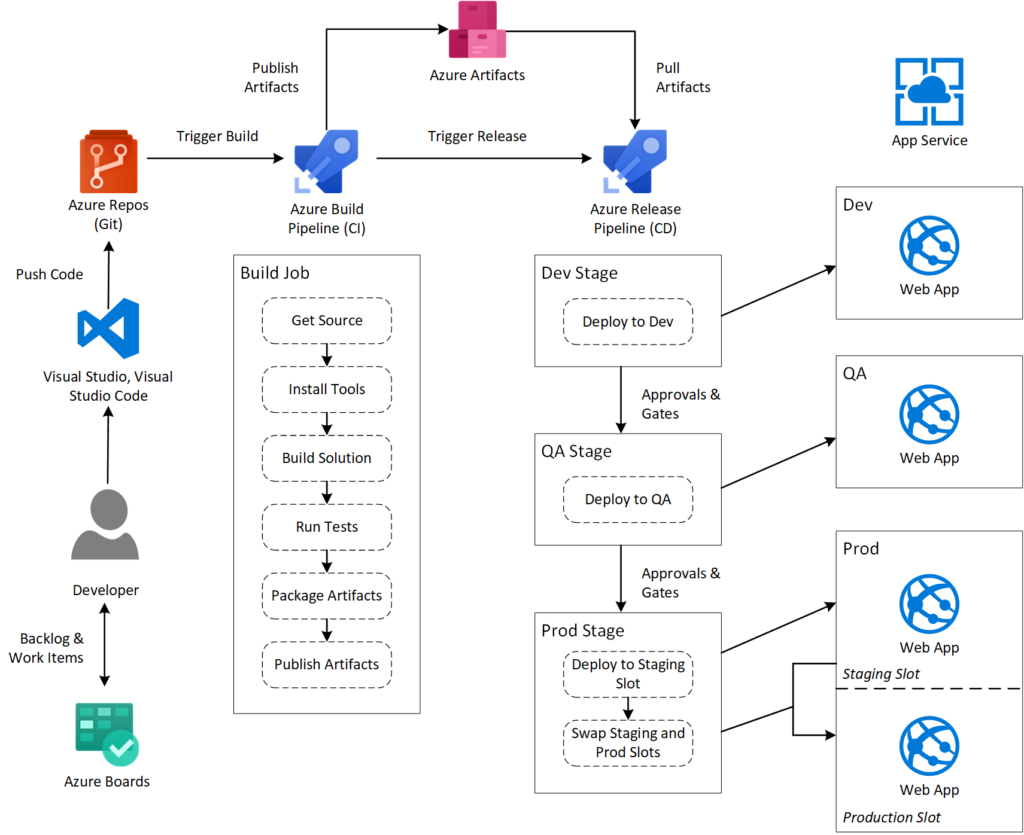
\includegraphics[width=13cm]{images/saiful/azure-devops-ci-cd-pipeline-workflow.png}
    \caption{Azure DevOps CI-CD workflow}
    \label{fig:azure-devops-ci-cd-pipeline-workflow}
\end{figure}

In Azure DevOps, developers manage and keep track of their tasks and backlogs by using the azure boards service. The source code is developed in a local environment. Azure provides seamless integration with most of the popular IDEs like VS Code, Intellij Idea, and Eclipse through extension. Whenever a new commit is pushed to the Azure Repos service, it triggers a new build job at Azure Pipelines. A build job can have many stages like installing tools, testing, and more. These steps in a build job can be defined manually by a developer in an azure CI pipeline. After the build is complete, the generated application artifacts are stored in the azure artifacts service. Continuous Delivery pipeline is also configured in the azure pipeline service. Whenever a CD pipeline is triggered, it fetches all the necessary artifacts from the azure artifacts service, and it deploys the application in a pre-configured environment. These environments are used to define and isolate development, QA, and production stages in a CI-CD pipeline. These environments are actually stored as a resource group in the Azure portal. \footnote{\url{https://www.veritis.com/wp-content/uploads/2019/02/azure-devops-ci-cd-pipeline-flow-veritis-1024x835.png}}

\begin{figure}[h]
    \centering
    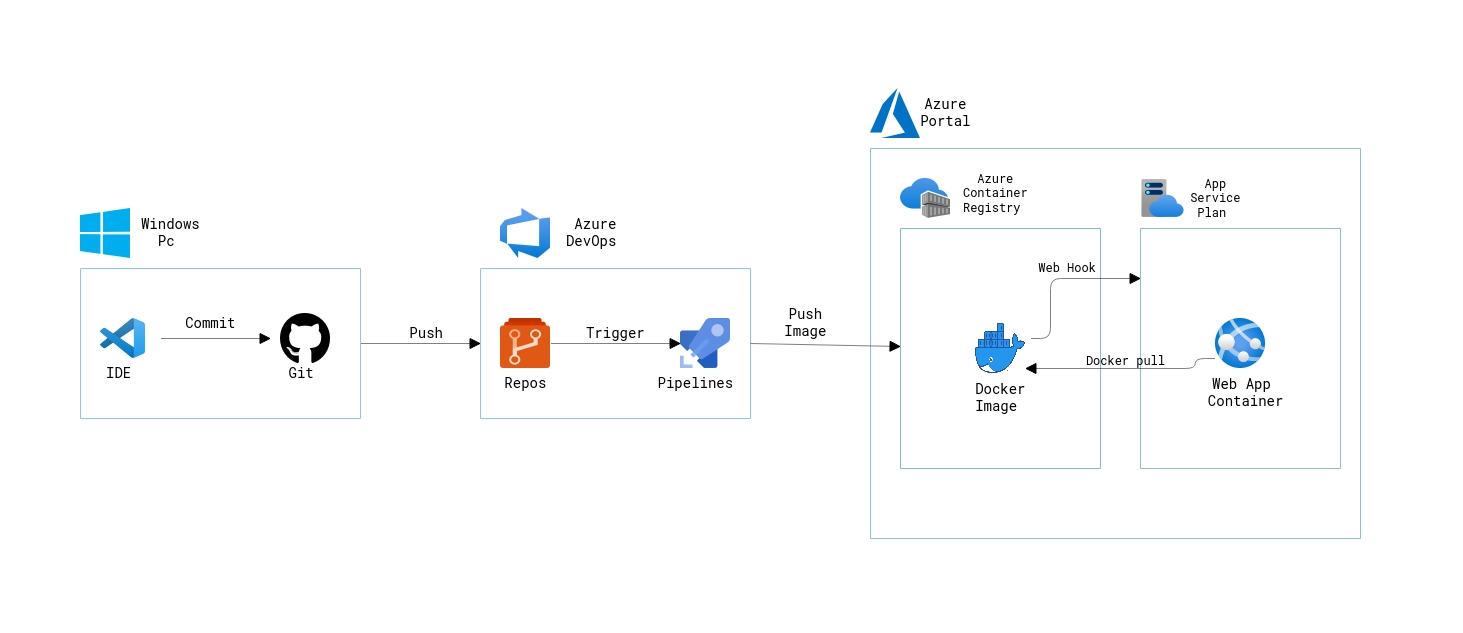
\includegraphics[width=14cm]{images/saiful/Azure_pipeline_diagram_CD.png}
    \caption{Azure DevOps CD to Portal}
    \label{fig:azure-devops-ci-cd-portal}
\end{figure}

After CD pipelines are executed, the application is continuously deployed in the Azure portal. Figure-\ref{fig:azure-devops-ci-cd-pipeline-workflow} represents a CD-CD pipeline that generates a containerized Docker image of the application. This image can be configured to be automatically stored in a public registry like DockerHub, or Azure's own private registry Azure container registry. From where other deployment platforms like Azure App service pan, Azure Kubernetes Service (AKS), Azure container instance (ACI) pulls the image through webhooks and deploys the application. All of these steps can be defined by using the azure pipeline's service, which will automate the entire system.

%

\subsubsection{Advantages [Md Saiful Ambia Chowdhury]}
%
Since Azure DevOps is a Software-as-a-service(SaaS) product, it has many advantages like :\footnote{\url{https://www.softacom.com/en_azure_devops}}
1. No manual infrastructure maintenance is needed. 2. It is much more intuitively clear and user-friendly in comparison to similar platforms. 3. Users don’t need to worry about upgrading or patching up the tool-chain. Thus massive organizations using the DevOps service will not experience any slowdown in CI-CD pipelines.
  
 In Azure DevOps, tasks are categorized based on the nature of the operation. For Instance, Build tasks, Utility tasks, Deploy tasks, etc. This facilitates the user in adding desired tasks to their pipeline in an organized manner.\footnote{\url{https://ymedialabs.medium.com/the-pros-and-cons-of-jenkins-vs-azure-devops-469c66140b4d}}
 It also provides the option to encapsulate a sequence of tasks, already defined in a pipeline, into a single reusable task, just like any other task.
   The Azure DevOps is platform agnostic. Which means, it is designed to run on any platform (Linux, macOS, and Windows) or language (e.g., Android, C/C++, Node.js, Python, Java, PHP, Ruby, .Net, and iOS apps).
Similarly, it is cloud agnostic. That means, Azure DevOps can work in conjunction with AWS and GCP or even with an on-premise server. 
%

\subsubsection{Disadvantages [Md Saiful Ambia Chowdhury]}
%
Azure Pipeline workflow is straightforward. It can’t if-else or switch-case constructions. This makes it more difficult to develop complex workflows. If the project requires exploratory testing such as alpha, beta testing, then the cost structure becomes expensive. Moreover, Documentations of azure are not always up-to-date and sometimes missing. Integration with non-Microsoft tools sometimes can be problematic. 

%

\subsubsection{Price Plans [Md Saiful Ambia Chowdhury]}
%
   Azure DevOps offers two different plans for purchase : 1. Basic Plan, and 2. Basic + Test Plans. The Basic Plan is free for up-to 5 users, from 6 users on-wards the organization will be charged 6 USD per user every month. Basic + Test Plans costs 52 USD per user per month. 
%

%
\subsection{Comparison Azure vs AWS vs Google Cloud [Md Anisul Haque]}
%

Azure was first developed in 2010(renamed as 'Microsoft Azure' in 2014), AWS was developed in 2006 and Google Cloud started in 2011.\footnote{https://intellipaat.com/blog/aws-vs-azure-vs-google-cloud/} For computing service Azure uses virtual machines, whereas AWS uses Elastic Compute Cloud(EC2) and google cloud use compute engine. Both Azure and AWS instances are auto-scaling and Google Cloud has instance grouping\cite{articleComparison}. Azure uses DevOps/GitHub , AWS code commit and Google Cloud uses Cloud Source Repositories for version control. In comparison to serverless computing, Azure used Azure functions.
Meanwhile, AWS used Lambda. However, Google cloud used cloud functions. They also have different pricing schemes. In a nutshell, it is much complex to choose this kind of solution. It mainly depends on the application and consumer needs, though they have similar mainly virtue of workings.  


\section{Continuous Integration in Cloud Native architecture [Md Jahidul Haque]}\label{sec:jahidul_sec_1}

Software releasing process can be procedural in the conventional software development life-cycle(SDLC). In traditional SDLC, the software development mostly depends on the different development teams working on the different parts of the same project. Ideally, developers need to collaborate between themselves to mitigate the knowledge gaps to ensure a successful release of the software. During the software releasing process, the code review of any changes in the existing software is very crucial in SDLC. After reviewing the code by the code review team, the new changes in the code is inspected but he testing team for the quality assurance of the new changes. This new changes is then passes through various unit testing and  integration testing by the testing team. Furthermore, the QA passed patch of the software is handed over the deployment team who are responsible for the releasing the new version of the software. This involves DevOps tasks for the deployment team. The DevOps engineers create and manage different cloud services to provision and scale the software deployment during the release. After Provisioning and scaling the new version of the software is released. 

The cloud-native architecture suggest software release via public clouds like AWS, Google Cloud or the Microsoft Azure. Also, this approach overcome the various hurdles of setting up on-premise infrastructure. Yet, the public cloud based software development  suffers vendor lock-in issues. In the traditional way of software release described in the previous paragraph, managing cloud-native application is much tougher to provision and scale manually for the deployment team. This creates time lagging in SDLC for any new modification of the software. In this particular case, CI/CD comes in practice among the software development community. CI/CD stands for continuous integration and continuous deployment/delivery. In this novel approach, SDLC can achieve more granular gain from the resource optimization during the release process of the software. Moreover, this process helps developers to automate tests and make QA process more free from human errors. 

The Continuous integration of the cloud-native application means the automation of the software releasing process via automation of various SDLC processes. For example, the automation in the repository management in continuous integration reefers to development of automation scripts that can automatically handle any new changes of the repository of a application code-base. These automation scripts can be handled different technologies like Gihub Actions, GitLab CI/CD, Jenkins, CircleCI. For public cloud like the AWS or the Azure, Github or GitLab can be used by the developers to developer automation scripts for managing the repository in the case of modification or new release of the software.

In this report we will talk about the implementation of the automation of the software release for the spring-boot application. At the beginning of the implementation we have a spring-boot application which have several services exposed and the application is using Gradle package management for dependency management. In our implementation, we will implement continuous by developing a CI pipeline for integrating the application in AWS cloud services. Our implementation involves two major parts: continuous integration and continuous deployment/delivery. 








\section{Continuous Deployment/Delivery in cloud-native architecture [Md Jahidul Haque]}

Continuous deployment in SDLC involves the automation of the software release process via configuration scripts in deployment automation technologies. Github offers Github Actions feature which is the main platform for describing the continuous deployment process. Gihub offers developers to develop their release process via Github's own domain specific language (DSL). Github's DSL supports {{.yml}} scripts to write github workflows. Github Workflow enables various jobs for deployment inside the development environment. Developers can manage their repository and create automated tasks to serialize the batch processes during the deployment. The main purpose of this continuous deployment is initiate the continuous integration smoothly without the manual configuration of the repository. After conducting all the acceptance testing the automation jobs can also create new dependencies via the {{.yml}} files. But the continuous deployment lacks the infrastructure automation which brings the manual configuration of the public cloud infrastructure. This technological need brings the concept of continuous delivery.

Continuous delivery refers to deployment automation when developer is able to automate the cloud infrastructure via the infrastructure automation objects. This enables the developer to manage,provision and scale the whole infrastructure which is needed for their developed software. In the infrastructure automation process, Github Action also involves for managing the pipeline where services in AWS are responsible for creating the infrastructure objects. The main technology of continuous delivery is CloudFormation from AWS. CloudForamtion is a complete infrastructure automation tool for continuous delivery of a software. 

In summary, the CD pipeline of the SDLC means the automation of the release processes which are related with automatic deployment environment, network configuration and infrastructure object creation. For automating deployment environment, Github actions can be used to describe the environment definitions to create resources that are needed for the application. Then other batch jobs execute deployment environment and test the application via acceptance testing. After successful deployment, the infrastructure objects creation are defined via CloudFomation's  cloud development kit(CDK). In this CDK, we can define Java classes for describing the infrstrructure objects and then that objects can be compiled via AWS's CLI. All the infrastucture automation commands is included in the Github actions so that infrastructure objects can automatically be created via {{.yml}} scripts.

In this report, we briefly define the our implementation of AWS based cloud-native
pipeline automation. In the starting stage of the pipeline we integrated Continuous integration which is described in section ~\ref{sec:jahidul_sec_1} and then we implemented Continuous deployment/delivery described in this section.  




\section{Implementation of CI/CD pipeline via GitHub Actions for AWS [ Md Yousuf Ali Khan]}\label{sec:chapter_1}
For Continuous Integration and Continuous deployment, we used GitHub actions. Github action is event-driven means we can run series of tasks in a reaction to a specific event. An event triggers a workflow, which contains a job. A job consists of multiple steps which control the order of actions.

Workflows can contain multiple jobs which can be triggered or scheduled based on events. An event can be internal or external. A job is a set of steps. Workflow with multiple jobs by default will run those jobs on parallel, but we can change this behavior and make it sequential by making a job dependent on other jobs. This will also ensure that if a parent job fails, all the other jobs dependent on that job will not even run. The main goal of a Step is to run commands in a job. In comparison, actions are standalone commands that steps are made of. 

While designing our pipeline, we considered any push to our main branch as an event that will trigger our workflow. One of our starting jobs is to building our application and run the tests. If our tests failed or any kind of error occurred during the building of our application, we will generate a report consisting of the stacktrace and publish it as an artifact that can be downloaded anytime for debugging purposes. We also introduced caching for our application packages which will speed up the time to run our pipeline. Next, We will create a docker repository in AWS ECR for our application images. We had to provide our AWS account access key and secret access key for doing so from our pipeline. We used another feature of Github called secrets to provide those values, enabling us to use this sort of private value without exposing it. We created four of those secrets for our account id, access key id, secret access key, and AWS region. The commands that we had to run for our CDK to create and deploy our resources to AWS were becoming quite long. So we decided to create an npm repo inside the root of our CDK folder, which will help us hide those long commands behind short npm commands. Some of our CDK commands need variable parameters even that we can pass from our npm commands, making our pipeline much more readable. Also, we made this job depend on our pipeline's build job, which ensures that we will not run this job if our build job fails for any reason. The following job of our pipeline will create a network stack in our AWS account. We provide all the necessary secrets for building that stack and provide the environment as an argument in our npm command, enabling us to create different deployment environments for our application. The next step is to create a database stack. For deploying that stack, we passed two parameters, environment and application name to our CDK so that it can create a database for using that application name and using the environment variable that will be able to create that database to a specific environment. Our pipeline's last job is to build our application image and push that one to our AWS ECR repository that we created in one of the previous steps. We will build a new image for every release of our application and tag it with a unique name, which we will create using the current date and time along with the unique SHA value for that commit. Finally, we will clear the old parameter stacks that we used for publishing some of the resources ids and other properties that we wanted to share between multiple stacks.

In the next subsections, we will briefly  describe the implementation stages of our implementation of the automated software release in AWS cloud. 


\subsection{Overview of the implementation architecture[Md Jahidul Haque]}\label{sec:arch-aws}
In order to implement the CI/CD pipeline for our spring boot application, we needed a technology to choose for the repository management. In this case, we used the GitHub Actions for the repository management. Unlike codeCommit from AWS, Github Action is free to use and this way we cover up our cost of implementation. We have used GitHub's DSl to setup the configuration scripts in {{.yml}} files. 

The CI is managed via the {{.yml}} file of our code base. To simplify our tasks for automating the infrastructure objects we used node package manager(npm) to setup the necessary commands for the pipeline.

The CD pipeline of the SDLC means the automation of the release processes which are related with automatic deployment environment, network configuration and infrastructure object creation. For automating deployment environment, Github actions can be used to describe the environment definitions to create resources that are needed for the application. Then other batch jobs execute deployment environment and test the application via acceptance testing. 

After successful deployment, the infrastructure objects creation are defined via CloudFomation's  cloud development kit(CDK). In this CDK, we can define Java classes for describing the infrastructure objects and then that objects can be compiled via AWS's CLI. All the infrastucture automation commands is included in the Github actions so that infrastructure objects can automatically be created via {{.yml}} scripts.











In our implementation, we used several technology to automate the software release. Beside using Github Actions, we also used docker file to create deployment environment and AWS CloudFormation for continuous delivery. The figure ~\ref{fig:ci-cd} describes all the github steps that we created in the pipeline implementation for AWS based spring boot application.

\begin{figure}[h]
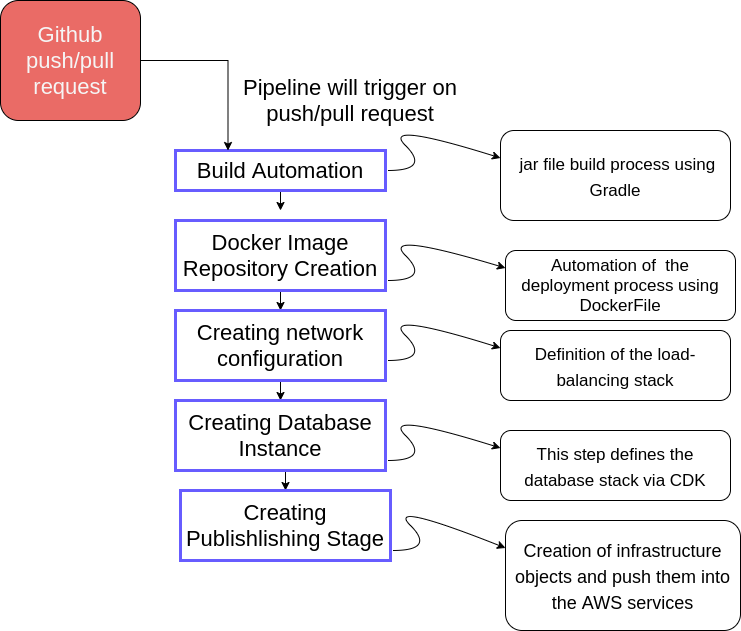
\includegraphics[scale=0.60]{images/jahidul/arch_ci_cd.png}
\centering
\caption{The {{CI\CD}} pipeline Architecture for AWS Cloud-native Application}
\label{fig:ci-cd}
\end{figure}

In the Figure.~\ref{fig:ci-cd} the triggering mechanism is indicated which briefs the pipeline orchestration on push or pull request of the project's repository. In order to maintain branch operation we defined the designated branch to pick in the job definition so that github workflow can checkout the defined branch in the {{.yml}} file. When the push is triggred in the designated branch in the {{.yml}} file, the build process starts as shown in the figure \ref{fig:ci-cd} and then other task are initiated accordingly. In this project, we implement five key tasks for the spring-boot application. For deployment automation at first we implemented a CI/CD pipeline architecture using Github Actions. Then we secured our DNS of the service via implementing the SSL certificated via letsencrypt inside the AWS ECS container. After securing our DNS we developed a new service of the application to test the whole pipeline. During the development of the service we have created integration tests, unit tests using JUNIT5. In this implementation, we also enable PostgreSQL configurations inside the AWS's RDS container for maintaining the persistence data. After developing the new modification of the software, we implemented the whole infrastructure automation using the CDK of AWS's CloudFormation.
\subsection{Build, Deployment and release via CI/CD pipeline in AWS[ Md Yousuf Ali Khan]}\label{sec:build-task-aws}
We used the AWS ECS (Amazon Elastic Container Service) service to deploy our application, a fully managed container orchestration service that enables us to deploy, manage, and scale containerized applications. We created a new docker image for every new release of our application and uploaded that docker image into Amazon ECR (Elastic Container Registry), which is a private container registry. AWS ECS uses that container image, takes care of the scaling of our application, and manages our containers for availability. By using AWS ECS, we will not have to worry about the scalability of our application. In figure~\ref{sec:build-task-aws} the build job for creating a build for the newly modified code in the repository is presented.

\begin{figure}[h]
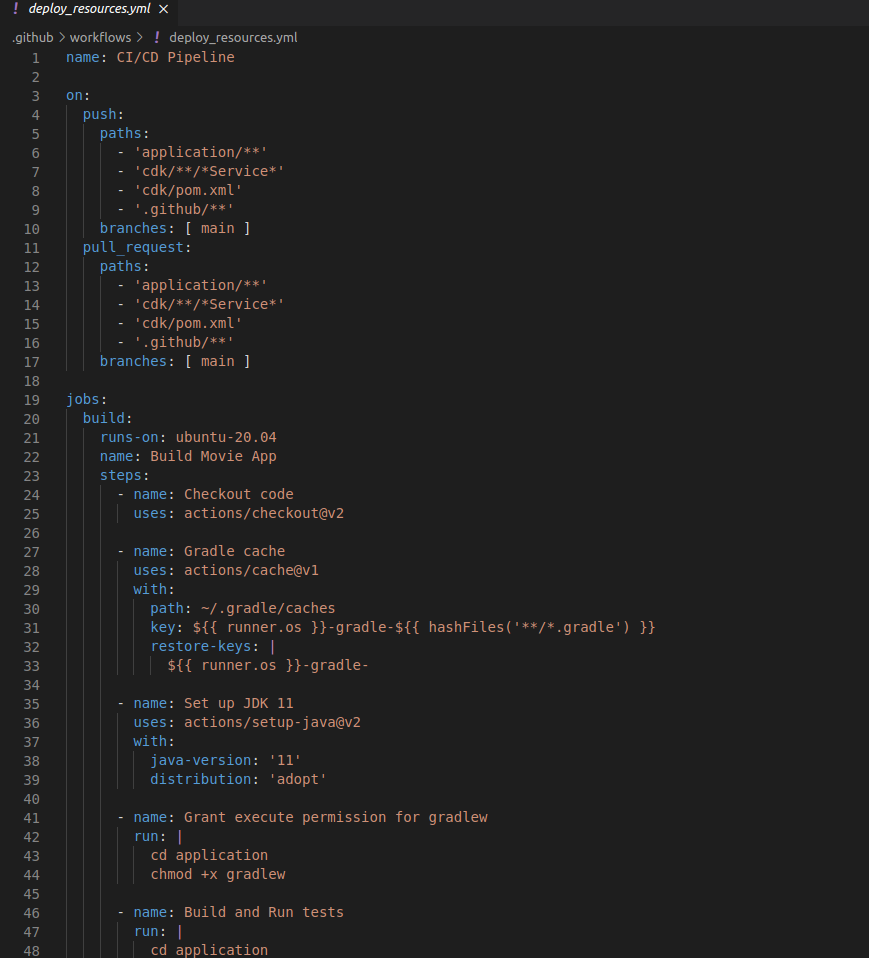
\includegraphics[scale=0.40]{images/yousuf/build-job-aws-github.png}
\centering
\caption{The {{CI\CD}} pipeline build task in Github workflow file}
\label{fig:ci-cd-build-task}
\end{figure}





\subsection{Implementation of the New features and automated testing in Spring-boot Application[Md Yousuf Ali Khan] }\label{sec:feture-imp-spring-boot}

We created an actor page where normal users can only view all the existing actors but can not add new actors. However, if the user is an admin user, he/she can add new actors, which will be stored in the database. 

We used GitHub actions for running our unit tests in both staging and production deployment pipelines. In our pipeline, while building and running the unit tests, we will create a report as a zip artifact that will contain all the stack traces for future investigations if there any error occurred. Any kind of failure in unit tests will also terminate all the following pipeline operations. 
%In the following paragraphs we will describe the implementation details of the new features: 


\subsection{AWS CloudFormation Stack Implementation [ Md Yousuf Ali Khan]}\label{sec:aws-cloudformation-stack}
As we choose AWS as our cloud provider, there were multiple options for implementing our IAAC. For example, we could use Terraform or AWS CloudFormation templates using JSON and YAML, but we found a better solution called AWS CDK(AWS Cloud Development Kit). AWS CDK is a software development framework for defining cloud infrastructure resources in code and deploying all those resources using AWS CloudFromation. In AWS CDK, we can write our infrastructure code in different programming languages like TypeScript, JavaScript, Python, Java, and C#. Even though TypeScript is the first language supported for developing AWS CDK applications, we choose Java as our AWS CDK language as our application was written in Java. We created a separate project for our infrastructure code in a folder called 'CDK.' Few significant benefits of using CDK are that we can use our object-oriented programming techniques to model your system using our desired programming language.
Furthermore, we can create and define high-level abstractions of our infrastructure, which will enable us to reuse those constructs in the future. We can even share or publish those constructs for public use.  A CDK construct is a basic building block of AWS CDK apps which is a single pre-configured CloudFormation resource or a stack that can be combined in any way to create any desired infrastructure. There are three different levels of constructs: Level 1 constructs, Level 2 constructs, and Level 3 constructs. Level 1 constructs are the direct equivalent of an underlying CloudFormation resource.
In contrast, Level 2 constructs consist of multiple Level 1 constructs; as a result, we can use those Level 2 constructs instead of creating all the Level 1 constructs manually by ourselves. Level 3 constructs provide the highest level of abstraction, also known as "patterns." Level 3 constructs mainly provide a built-in architecture pattern for our infrastructures. In our project, we used an open-source package that provides us with Level 2 and Level 3 constructs for our infrastructure. 

We created four different CloudFormation stacks to define our desired infrastructure. First, we will create a docker repository stack which creates a docker repository in AWS ECR for our application's docker images. Then, with every new release of our application, we will create a docker image with a tag for it and push it to this repository. Afterward, we will create a network stack that will create a VPC with a public and private subnet. In this stack, we will also create a loadbalancer (AWS ALB) which will be inside our public subnet, and forward all the incoming requests to the ECS cluster, which will actually run our application image inside a container environment. The private subnet will not be reachable from the outside world. Only from the public subnet will be able to communicate with any resources inside of this subnet. We will put our database inside of this subnet. That will ensure that no one will be able to access our database from outside, which is one of our project requirements.

We will create a database stack that will create a PostgreSQL database which will be used as the persistence layer of our application. As this database will be placed inside the private subnet, it will not be accessible from outside.

Finally, We will create a service stack that will create an ECS service and an ECS Task. As we only have one application to deploy, we will have only one ECS task, which will contain our application image. Our ECS service will contain a single ECS task. This ECS service will take care of the automatic scaling of our application in case of increasing loads. In case of increasing load, it will spin up EC2 compute instances for hosting the configured docker image defined on the ESC task. Behind the scene, ECS will use AWS Faragate, which is a serverless compute engine for containers. It will also take care of shutting down all those extra containers when there is not enough load. In this way, we will never have to worry about running out of computing power in case of extreme loads. Our application will always be up and running while we do not need to pay for any extra resources as our resources will be scaled based on the load.

For Continuous Integration and Continuous deployment, we used GitHub actions. Github action is event-driven means we can run series of tasks in a reaction to a specific event. An event triggers a workflow, which contains a job. A job consists of multiple steps which control the order of actions.

Workflows can contain multiple jobs which can be triggered or scheduled based on events. An event can be internal or external. A job is a set of steps. Workflow with multiple jobs by default will run those jobs on parallel, but we can change this behavior and make it sequential by making a job dependent on other jobs. This will also ensure that if a parent job fails, all the other jobs dependent on that job will not even run. The main goal of a Step is to run commands in a job. In comparison, actions are standalone commands that steps are made of. 

While designing our pipeline, we considered any push to our main branch as an event that will trigger our workflow. One of our starting jobs is to building our application and run the tests. If our tests failed or any kind of error occurred during the building of our application, we will generate a report consisting of the stacktrace and publish it as an artifact that can be downloaded anytime for debugging purposes. We also introduced caching for our application packages which will speed up the time to run our pipeline. Next, We will create a docker repository in AWS ECR for our application images. We had to provide our AWS account access key and secret access key for doing so from our pipeline. We used another feature of Github called secrets to provide those values, enabling us to use this sort of private value without exposing it. We created four of those secrets for our account id, access key id, secret access key, and AWS region. The commands that we had to run for our CDK to create and deploy our resources to AWS were becoming quite long. So we decided to create an npm repo inside the root of our CDK folder, which will help us hide those long commands behind short npm commands. Some of our CDK commands need variable parameters even that we can pass from our npm commands, making our pipeline much more readable. Also, we made this job depend on our pipeline's build job, which ensures that we will not run this job if our build job fails for any reason. The following job of our pipeline will create a network stack in our AWS account. We provide all the necessary secrets for building that stack and provide the environment as an argument in our npm command, enabling us to create different deployment environments for our application. The next step is to create a database stack. For deploying that stack, we passed two parameters, environment and application name to our CDK so that it can create a database for using that application name and using the environment variable that will be able to create that database to a specific environment. Our pipeline's last job is to build our application image and push that one to our AWS ECR repository that we created in one of the previous steps. We will build a new image for every release of our application and tag it with a unique name, which we will create using the current date and time along with the unique SHA value for that commit. Finally, we will clear the old parameter stacks that we used for publishing some of the resources ids and other properties that we wanted to share between multiple stacks.



